\documentclass{standalone}
\usepackage{tikz}
\usetikzlibrary{patterns, positioning}


\begin{document}
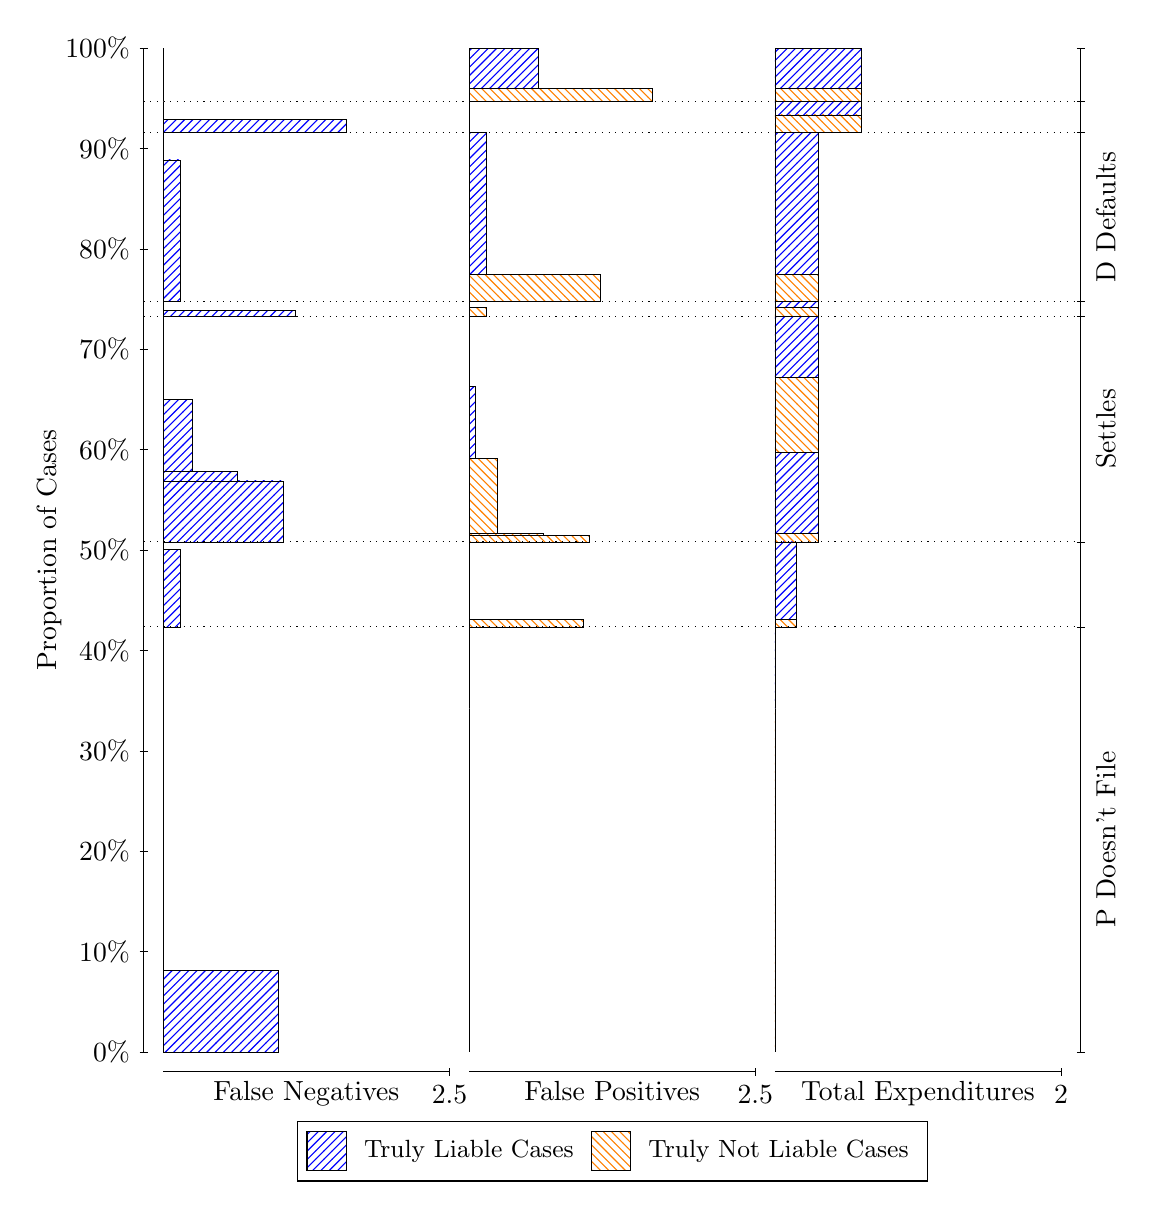
\begin{tikzpicture}
\draw[black, very thin] (1.5,1.75) -- (1.5,14.5);
\node[rotate=90, text=black, anchor=center] at (0.3, 8.125) {Proportion of Cases};
\draw[black, very thin] (1.45,1.75) -- (1.55,1.75);
\node[text=black, anchor=east] at (1.45, 1.75) {0\%};
\draw[black, very thin] (1.45,3.025) -- (1.55,3.025);
\node[text=black, anchor=east] at (1.45, 3.025) {10\%};
\draw[black, very thin] (1.45,4.3) -- (1.55,4.3);
\node[text=black, anchor=east] at (1.45, 4.3) {20\%};
\draw[black, very thin] (1.45,5.575) -- (1.55,5.575);
\node[text=black, anchor=east] at (1.45, 5.575) {30\%};
\draw[black, very thin] (1.45,6.85) -- (1.55,6.85);
\node[text=black, anchor=east] at (1.45, 6.85) {40\%};
\draw[black, very thin] (1.45,8.125) -- (1.55,8.125);
\node[text=black, anchor=east] at (1.45, 8.125) {50\%};
\draw[black, very thin] (1.45,9.4) -- (1.55,9.4);
\node[text=black, anchor=east] at (1.45, 9.4) {60\%};
\draw[black, very thin] (1.45,10.675) -- (1.55,10.675);
\node[text=black, anchor=east] at (1.45, 10.675) {70\%};
\draw[black, very thin] (1.45,11.95) -- (1.55,11.95);
\node[text=black, anchor=east] at (1.45, 11.95) {80\%};
\draw[black, very thin] (1.45,13.225) -- (1.55,13.225);
\node[text=black, anchor=east] at (1.45, 13.225) {90\%};
\draw[black, very thin] (1.45,14.5) -- (1.55,14.5);
\node[text=black, anchor=east] at (1.45, 14.5) {100\%};

\draw[black, very thin] (13.4,1.75) -- (13.4,14.5);
\draw[black, very thin] (13.35,1.75) -- (13.45,1.75);
\node[anchor=west] at (13.35, 1.75) {};
\draw[black, very thin] (13.35,7.1483) -- (13.45,7.1483);
\node[anchor=west] at (13.35, 7.1483) {};
\draw[black, very thin] (13.35,8.2288) -- (13.45,8.2288);
\node[anchor=west] at (13.35, 8.2288) {};
\draw[black, very thin] (13.35,11.096) -- (13.45,11.096);
\node[anchor=west] at (13.35, 11.096) {};
\draw[black, very thin] (13.35,11.281) -- (13.45,11.281);
\node[anchor=west] at (13.35, 11.281) {};
\draw[black, very thin] (13.35,13.427) -- (13.45,13.427);
\node[anchor=west] at (13.35, 13.427) {};
\draw[black, very thin] (13.35,13.82) -- (13.45,13.82);
\node[anchor=west] at (13.35, 13.82) {};
\draw[black, very thin] (13.35,14.5) -- (13.45,14.5);
\node[anchor=west] at (13.35, 14.5) {};

\draw[black, very thin, pattern color=blue, pattern=north east lines] (1.75,1.75) rectangle (3.2033,2.7834);
\draw[black, very thin, pattern color=orange, pattern=north west lines] (1.75,2.7834) rectangle (1.75,7.1483);
\draw[black, very thin, pattern color=blue, pattern=north east lines] (1.75,7.1483) rectangle (1.968,8.1293);
\draw[black, very thin, pattern color=orange, pattern=north west lines] (1.75,8.1293) rectangle (1.75,8.2288);
\draw[black, very thin, pattern color=blue, pattern=north east lines] (1.75,8.2288) rectangle (3.276,9.0034);
\draw[black, very thin, pattern color=blue, pattern=north east lines] (1.75,9.0034) rectangle (2.6947,9.1209);
\draw[black, very thin, pattern color=blue, pattern=north east lines] (1.75,9.1209) rectangle (2.1133,10.036);
\draw[black, very thin, pattern color=orange, pattern=north west lines] (1.75,10.036) rectangle (1.75,11.096);
\draw[black, very thin, pattern color=blue, pattern=north east lines] (1.75,11.096) rectangle (3.4213,11.171);
\draw[black, very thin, pattern color=orange, pattern=north west lines] (1.75,11.171) rectangle (1.75,11.281);
\draw[black, very thin, pattern color=blue, pattern=north east lines] (1.75,11.281) rectangle (1.968,13.08);
\draw[black, very thin, pattern color=orange, pattern=north west lines] (1.75,13.08) rectangle (1.75,13.427);
\draw[black, very thin, pattern color=blue, pattern=north east lines] (1.75,13.427) rectangle (4.0753,13.597);
\draw[black, very thin, pattern color=orange, pattern=north west lines] (1.75,13.597) rectangle (1.75,13.82);
\draw[black, very thin, pattern color=orange, pattern=north west lines] (1.75,13.82) rectangle (1.75,13.99);
\draw[black, very thin, pattern color=blue, pattern=north east lines] (1.75,13.99) rectangle (1.75,14.5);
\draw[black, very thin, pattern color=orange, pattern=north west lines] (5.6333,1.75) rectangle (5.6333,6.1149);
\draw[black, very thin, pattern color=blue, pattern=north east lines] (5.6333,6.1149) rectangle (5.6333,7.1483);
\draw[black, very thin, pattern color=orange, pattern=north west lines] (5.6333,7.1483) rectangle (7.0867,7.2479);
\draw[black, very thin, pattern color=blue, pattern=north east lines] (5.6333,7.2479) rectangle (5.6333,8.2288);
\draw[black, very thin, pattern color=orange, pattern=north west lines] (5.6333,8.2288) rectangle (7.1593,8.3089);
\draw[black, very thin, pattern color=orange, pattern=north west lines] (5.6333,8.3089) rectangle (6.578,8.3336);
\draw[black, very thin, pattern color=orange, pattern=north west lines] (5.6333,8.3336) rectangle (5.9967,9.2893);
\draw[black, very thin, pattern color=blue, pattern=north east lines] (5.6333,9.2893) rectangle (5.706,10.204);
\draw[black, very thin, pattern color=blue, pattern=north east lines] (5.6333,10.204) rectangle (5.6333,11.096);
\draw[black, very thin, pattern color=orange, pattern=north west lines] (5.6333,11.096) rectangle (5.8513,11.206);
\draw[black, very thin, pattern color=blue, pattern=north east lines] (5.6333,11.206) rectangle (5.6333,11.281);
\draw[black, very thin, pattern color=orange, pattern=north west lines] (5.6333,11.281) rectangle (7.3047,11.628);
\draw[black, very thin, pattern color=blue, pattern=north east lines] (5.6333,11.628) rectangle (5.8513,13.427);
\draw[black, very thin, pattern color=orange, pattern=north west lines] (5.6333,13.427) rectangle (5.6333,13.65);
\draw[black, very thin, pattern color=blue, pattern=north east lines] (5.6333,13.65) rectangle (5.6333,13.82);
\draw[black, very thin, pattern color=orange, pattern=north west lines] (5.6333,13.82) rectangle (7.9587,13.99);
\draw[black, very thin, pattern color=blue, pattern=north east lines] (5.6333,13.99) rectangle (6.5053,14.5);
\draw[black, very thin, pattern color=orange, pattern=north west lines] (9.5167,1.75) rectangle (9.5167,6.1149);
\draw[black, very thin, pattern color=blue, pattern=north east lines] (9.5167,6.1149) rectangle (9.5167,7.1483);
\draw[black, very thin, pattern color=orange, pattern=north west lines] (9.5167,7.1483) rectangle (9.7892,7.2479);
\draw[black, very thin, pattern color=blue, pattern=north east lines] (9.5167,7.2479) rectangle (9.7892,8.2288);
\draw[black, very thin, pattern color=orange, pattern=north west lines] (9.5167,8.2288) rectangle (10.062,8.3336);
\draw[black, very thin, pattern color=blue, pattern=north east lines] (9.5167,8.3336) rectangle (10.062,9.3661);
\draw[black, very thin, pattern color=orange, pattern=north west lines] (9.5167,9.3661) rectangle (10.062,10.322);
\draw[black, very thin, pattern color=blue, pattern=north east lines] (9.5167,10.322) rectangle (10.062,11.096);
\draw[black, very thin, pattern color=orange, pattern=north west lines] (9.5167,11.096) rectangle (10.062,11.206);
\draw[black, very thin, pattern color=blue, pattern=north east lines] (9.5167,11.206) rectangle (10.062,11.281);
\draw[black, very thin, pattern color=orange, pattern=north west lines] (9.5167,11.281) rectangle (10.062,11.628);
\draw[black, very thin, pattern color=blue, pattern=north east lines] (9.5167,11.628) rectangle (10.062,13.427);
\draw[black, very thin, pattern color=orange, pattern=north west lines] (9.5167,13.427) rectangle (10.607,13.65);
\draw[black, very thin, pattern color=blue, pattern=north east lines] (9.5167,13.65) rectangle (10.607,13.82);
\draw[black, very thin, pattern color=orange, pattern=north west lines] (9.5167,13.82) rectangle (10.607,13.99);
\draw[black, very thin, pattern color=blue, pattern=north east lines] (9.5167,13.99) rectangle (10.607,14.5);
\draw[black, dotted] (1.5,7.1483) -- (13.4,7.1483);
\draw[black, dotted] (1.5,8.2288) -- (13.4,8.2288);
\draw[black, dotted] (1.5,11.096) -- (13.4,11.096);
\draw[black, dotted] (1.5,11.281) -- (13.4,11.281);
\draw[black, dotted] (1.5,13.427) -- (13.4,13.427);
\draw[black, dotted] (1.5,13.82) -- (13.4,13.82);
\draw[black, very thin] (1.75,1.5) -- (5.3833,1.5);
\node[text=black, anchor=north] at (3.5667, 1.5) {False Negatives};
\draw[black, very thin] (5.3833,1.45) -- (5.3833,1.55);
\node[text=black, anchor=north] at (5.3833, 1.45) {2.5};

\draw[black, very thin] (5.6333,1.5) -- (9.2667,1.5);
\node[text=black, anchor=north] at (7.45, 1.5) {False Positives};
\draw[black, very thin] (9.2667,1.45) -- (9.2667,1.55);
\node[text=black, anchor=north] at (9.2667, 1.45) {2.5};

\draw[black, very thin] (9.5167,1.5) -- (13.15,1.5);
\node[text=black, anchor=north] at (11.333, 1.5) {Total Expenditures};
\draw[black, very thin] (13.15,1.45) -- (13.15,1.55);
\node[text=black, anchor=north] at (13.15, 1.45) {2};

\node[text=black, centered, rotate=90] at (13.72, 4.4492) {P Doesn't File};

\node[text=black, centered, rotate=90] at (13.72, 9.6626) {Settles};

\node[text=black, centered, rotate=90] at (13.72, 12.354) {D Defaults};



\draw (7.449999999999999,1.5) node[draw=none] (baseCoordinate) {};
\begin{scope}[align=center]
        \matrix[scale=0.5, draw=black, below=0.5cm of baseCoordinate, nodes={draw}, column sep=0.1cm]{
            \node[rectangle, draw, minimum width=0.5cm, minimum height=0.5cm, pattern color=blue, pattern=north east lines] {}; &
            \node[draw=none, font=\small, text=black] (B) {Truly Liable Cases}; &
            \node[rectangle, draw, minimum width=0.5cm, minimum height=0.5cm, pattern color=orange, pattern=north west lines] {}; &
            \node[draw=none, font=\small, text=black] (B) {Truly Not Liable Cases}; \\
            };
\end{scope}

\end{tikzpicture}
\end{document}